\documentclass[11pt]{article}

\usepackage[review]{acl}
\usepackage{times}
\usepackage{latexsym}
\usepackage[T1]{fontenc}
\usepackage[utf8]{inputenc}
\usepackage{microtype}
\usepackage{graphicx}
\usepackage{booktabs}
\usepackage{xcolor}
\usepackage{algorithm}
\usepackage{algpseudocode}
\usepackage{multirow}
\usepackage{amsmath}
\usepackage{amssymb}
\usepackage{hyperref}

\newcommand{\scrag}{\textsc{Scrag}}
\newcommand{\rcrag}{\textsc{Rcrag}}
\newcommand{\supportbench}{\textsc{SupportBench}}
\newcommand{\todo}[1]{\textcolor{red}{\textbf{[TODO: #1]}}}

\title{SupportBot: Dual-RAG Case Mining for Grounded Technical Support \\ with the \supportbench{} Benchmark}
\author{Anonymous}

\begin{document}
\maketitle

\begin{abstract}
We present \textbf{SupportBot}, a technical support system that continuously mines structured problem--solution cases from community chat streams and retrieves from them to generate grounded responses. SupportBot introduces a \emph{dual-RAG architecture} that separates confirmed solutions (\scrag{}) from unconfirmed recommendations (\rcrag{}), enabling confidence-tiered retrieval with a promotion mechanism as recommendations are later confirmed. A unified multimodal buffer analysis extracts cases, detects solved arcs, and updates the knowledge base in a single LLM call per buffer window.

To enable reproducible evaluation of case-mining support systems, we release \supportbench{}, a multilingual benchmark of 60{,}000 messages from six technical support communities spanning three languages (Ukrainian, Spanish, English) and six domains. Each dataset contains naturally occurring troubleshooting exchanges with reply chains, media annotations, and anonymized user identifiers.

We evaluate SupportBot on \supportbench{} using an offline replay protocol that replicates real-time production behavior. On the Ardupilot-UA dataset (900/100 history/live split), SupportBot achieves a Score of 7.8/10 (quality $\times$ recall) with 100\% precision and 93\% recall, outperforming both a context-stuffing LLM baseline (7.2) and a chunked-RAG baseline (6.3). \supportbench{} provides the first public benchmark specifically designed for evaluating case-mining support bots across languages and domains.
\end{abstract}

\section{Introduction}

Every day, technical communities solve hundreds of problems that never make it into official documentation. A user reports a cryptic error, an expert suggests checking a configuration file, the user confirms it worked---and this exchange is lost in a chat log, invisible to the next person facing the same issue. Meanwhile, automated support systems continue querying static documentation that cannot capture these real-world solutions.

Standard retrieval-augmented generation (RAG) pipelines \citep{lewis2020rag,guu2020realm,borgeaud2022retro} assume access to a well-structured, static document corpus. This assumption breaks down in technical support contexts where: (1) critical knowledge exists only in ephemeral chat messages, (2) solutions emerge through multi-turn conversational arcs, (3) confirmation signals indicate which solutions actually worked, and (4) new issues arise faster than documentation updates.

SupportBot addresses these challenges through a \textbf{dual-RAG case mining architecture} that treats community conversations as a continuously growing, confidence-stratified knowledge base. The system operates two coupled processes: an offline mining pipeline that extracts structured cases and indexes them with confidence tiers, and an online response pipeline that retrieves from both confirmed and tentative cases alongside static documentation.

A critical design decision is the separation of \emph{confirmed} and \emph{unconfirmed} knowledge. In support communities, many responses are helpful suggestions that may or may not resolve the issue. Our dual-RAG architecture maintains two retrieval collections---\scrag{} (Solved Case RAG) for confirmed solutions and \rcrag{} (Recommendation Case RAG) for promising but unverified advice---with a promotion mechanism that moves recommendations to confirmed status when follow-up signals indicate success.

To evaluate case-mining support systems beyond a single proprietary deployment, we introduce \supportbench{}, a benchmark of 60{,}000 messages from six Telegram technical support groups in three languages (Ukrainian, Spanish, English) covering six distinct domains from embedded electronics to NAS networking. \supportbench{} is the first public benchmark designed specifically for this task.

Our contributions are:
\begin{enumerate}
    \item \textbf{Dual-RAG architecture}: A confidence-tiered retrieval system (\scrag{} + \rcrag{}) that separates confirmed solutions from unverified recommendations, with a promotion mechanism that tracks knowledge maturation.
    \item \textbf{Unified multimodal buffer analysis}: A single LLM call per buffer window that jointly performs case extraction, solved-arc detection, case promotion, and buffer update---replacing the prior cascade of $1 + N + M$ separate calls.
    \item \textbf{\supportbench{} benchmark}: A multilingual, multi-domain benchmark of 60K messages from six technical support communities, released for reproducible evaluation of case-mining systems.
    \item \textbf{Empirical validation}: Evaluation on \supportbench{} showing SupportBot achieves a Score of 7.8/10 with 100\% precision and 93\% recall, outperforming both a context-stuffing LLM baseline (+8\%) and a chunked-RAG baseline (+23\%).
\end{enumerate}

\section{System Architecture}

\begin{figure*}[t]
    \centering
    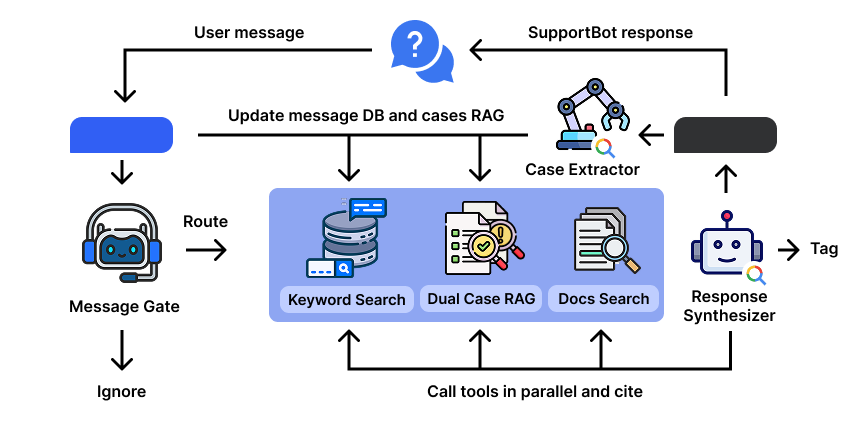
\includegraphics[width=0.95\textwidth]{algorithm.png}
    \caption{SupportBot architecture. Messages flow through a buffer window into the unified multimodal analysis, which extracts cases into \scrag{} (confirmed) or \rcrag{} (tentative). The response pipeline retrieves from both collections with confidence-weighted ranking, alongside documentation and conversation context.}
    \label{fig:architecture}
\end{figure*}

Figure~\ref{fig:architecture} illustrates the SupportBot architecture, which consists of three coupled components: unified buffer analysis, dual-RAG indexing, and multi-source response generation.

\subsection{Unified Multimodal Buffer Analysis}

The system maintains a sliding buffer of recent messages (300 messages / 7 days). Rather than processing messages individually, SupportBot performs a \emph{single unified LLM call} per buffer update that jointly handles all extraction tasks:

\begin{algorithm}[t]
\caption{Unified Buffer Analysis}
\label{alg:buffer}
\begin{algorithmic}[1]
\Require Buffer $B$ (text + images), \scrag{} index $\mathcal{S}$, \rcrag{} index $\mathcal{R}$
\State $\mathcal{I} \gets$ \Call{InterleavedContent}{$B$} \Comment{Text + images}
\State $\langle C_s, C_r, P, U \rangle \gets$ \Call{UnifiedLLM}{$\mathcal{I}$}
\For{each case $c \in C_s$} \Comment{Confirmed cases}
    \State $\mathcal{S} \gets \mathcal{S} \cup \{c\}$
\EndFor
\For{each case $c \in C_r$} \Comment{Recommendations}
    \State $\mathcal{R} \gets \mathcal{R} \cup \{c\}$
\EndFor
\For{each promotion $p \in P$} \Comment{Confirmed recommendations}
    \State $\mathcal{R} \gets \mathcal{R} \setminus \{p\}$; $\mathcal{S} \gets \mathcal{S} \cup \{p\}$
\EndFor
\State $B \gets$ \Call{ApplyUpdates}{$B, U$}
\end{algorithmic}
\end{algorithm}

Algorithm~\ref{alg:buffer} shows the unified analysis procedure. The LLM receives the full buffer content---including interleaved images (screenshots, error photos, configuration files)---and produces four outputs simultaneously:
\begin{itemize}
    \item $C_s$: New \textbf{solved cases} with confirmed resolutions
    \item $C_r$: New \textbf{recommendation cases} with promising but unverified advice
    \item $P$: \textbf{Promotions} of existing recommendations now confirmed by user follow-up
    \item $U$: \textbf{Buffer updates} (metadata, tag assignments)
\end{itemize}

This unified approach replaces a prior cascade of separate calls (1 gate classifier + $N$ case extractors + $M$ status updaters), reducing both latency and cost while improving coherence across extraction decisions.

\subsection{Dual-RAG: \scrag{} and \rcrag{}}
\label{sec:dualrag}

The core architectural innovation is maintaining two separate ChromaDB collections for confirmed and tentative knowledge:

\paragraph{\scrag{} (Solved Case RAG).} Contains cases where a clear problem--solution arc has been identified and the solution was confirmed by the original asker or through explicit success signals (e.g., ``works now'', ``that fixed it'', positive reactions). These cases are indexed with high retrieval priority.

\paragraph{\rcrag{} (Recommendation Case RAG).} Contains cases where an expert provided a plausible solution but no explicit confirmation was received. This includes: (a) detailed technical advice without follow-up, (b) solutions from experienced users with no response from the asker, and (c) partially confirmed fixes (``seems better but not sure'').

\paragraph{Promotion Mechanism.} When subsequent messages confirm a previously tentative recommendation, the unified buffer analysis detects this and promotes the case from \rcrag{} to \scrag{}. This models the natural lifecycle of community knowledge: advice starts as tentative, gains evidence through use, and eventually becomes established.

Each case contains structured fields:
\begin{itemize}
    \item \textbf{Problem}: Title and detailed description of the issue
    \item \textbf{Solution}: Step-by-step resolution or recommendation
    \item \textbf{Tags}: Technical topic labels for faceted retrieval
    \item \textbf{Evidence}: Supporting images, error messages, configurations
    \item \textbf{Status}: \texttt{solved} $|$ \texttt{recommendation} $|$ \texttt{archived}
\end{itemize}

Cases are embedded using Gemini embeddings and indexed in their respective ChromaDB collections. At retrieval time, results from both collections are returned with their confidence tier clearly marked, allowing the response generator to appropriately hedge recommendations.

\subsection{Response Generation Pipeline}

\begin{algorithm}[t]
\caption{Confidence-Tiered Response Generation}
\label{alg:response}
\begin{algorithmic}[1]
\Require Query $q$, \scrag{} $\mathcal{S}$, \rcrag{} $\mathcal{R}$, docs $\mathcal{D}$, history $H$
\State $g \gets$ \Call{GateClassifier}{$q$}
\If{$g = \text{NOISE}$}
    \State \Return $\varnothing$
\EndIf
\State $R_s \gets$ \Call{Retrieve}{$q, \mathcal{S}, k$} \Comment{Confirmed cases}
\State $R_r \gets$ \Call{Retrieve}{$q, \mathcal{R}, k$} \Comment{Recommendations}
\State $R_d \gets$ \Call{Retrieve}{$q, \mathcal{D}, k$} \Comment{Documentation}
\State $R_h \gets$ \Call{GetHistory}{$H$} \Comment{Recent context}
\State $R \gets$ \Call{RankAndMerge}{$R_s, R_r, R_d, R_h$}
\If{$|R| = 0$ \textbf{or} \Call{LowConfidence}{$q, R$}}
    \State \Return \Call{Abstain}{} \Comment{Escalate to human}
\EndIf
\State \Return \Call{Generate}{$q, R$} \Comment{With tier-aware citations}
\end{algorithmic}
\end{algorithm}

Algorithm~\ref{alg:response} describes the response pipeline. The key difference from standard RAG is \textbf{confidence-tiered ranking}: results from \scrag{} receive higher weight than \rcrag{} results, and the generator is instructed to mark recommendation-sourced information as tentative. Citations distinguish between ``confirmed solution from case \#X'' and ``community recommendation (unverified) from case \#Y''.

\section{\supportbench{}: A Multilingual Support Benchmark}
\label{sec:supportbench}

Existing benchmarks for dialogue systems and question answering do not adequately capture the challenges of technical support case mining. Forum datasets like MSDialog \citep{qu2018analyzing} and AskUbuntu \citep{lei2017semi} contain pre-structured threads with clear question--answer boundaries, while SupportBot must operate over unstructured group chat streams where problem boundaries are implicit and conversations interleave. To address this gap, we introduce \supportbench{}.

\subsection{Dataset Collection}

We collected 10{,}000 recent messages from each of six public Telegram technical support groups, selected to maximize diversity along three axes:

\paragraph{Language diversity.} We include groups in Ukrainian (UK), Spanish (ES), and English (EN), with two Ukrainian, two Spanish, and two English groups. This tests whether case mining generalizes across languages with different morphological complexity and technical vocabulary.

\paragraph{Domain diversity.} The six groups cover distinct technical domains: UAV/drone systems, networking infrastructure, smart home automation, NAS/networking, IoT firmware, and ad-blocking/DNS. Each domain has characteristic problem types, solution patterns, and media usage.

\paragraph{Interaction diversity.} Groups naturally vary in reply density (33--83\% reply rate), media usage (5--12\% of messages), thread structure (average thread sizes 3.1--17.0 messages), and message verbosity (median length 29--79 characters).

\subsection{Data Processing}

Messages are exported via the Telegram API using Telethon, then converted to a unified format matching SupportBot's production schema. Each message contains:
\begin{itemize}
    \item Unique message ID, group identifier, and millisecond timestamp
    \item Anonymized sender hash (SHA-256 of Telegram user ID)
    \item Message body text and media type annotation (\texttt{photo}, \texttt{video}, \texttt{document}, or \texttt{null})
    \item Reply-to reference (resolved within the export window)
\end{itemize}

Sender identities are irreversibly anonymized. No message content is modified. Media type annotations are preserved but binary media files are not distributed; future versions may include opt-in image subsets with additional consent.

\subsection{Dataset Statistics}

\begin{table*}[t]
\centering
\small
\begin{tabular}{llrrrrr}
\toprule
\textbf{Dataset} & \textbf{Lang} & \textbf{Msgs} & \textbf{Users} & \textbf{Reply\%} & \textbf{Q\&A} & \textbf{Media} \\
\midrule
Ardupilot-UA   & UK & 10{,}000 & 319  & 51.8 & 4{,}067 & 1{,}440 \\
MikroTik-UA    & UK & 10{,}000 & 205  & 55.4 & 4{,}466 & 884 \\
Domotica-ES    & ES & 10{,}000 & 530  & 58.3 & 5{,}171 & 736 \\
NASeros-ES     & ES & 10{,}000 & 761  & 46.5 & 3{,}980 & 495 \\
Tasmota-EN     & EN & 10{,}000 & 1{,}237 & 31.5 & 2{,}663 & 903 \\
AdGuard-EN     & EN & 10{,}000 & 954  & 46.2 & 3{,}994 & 1{,}049 \\
\midrule
\textbf{Total} & 3  & \textbf{60{,}000} & \textbf{4{,}006} & 48.3 & \textbf{24{,}341} & \textbf{5{,}507} \\
\bottomrule
\end{tabular}
\caption{\supportbench{} dataset statistics. \textbf{Q\&A}: messages with reply chains where the reply body $>$20 characters. \textbf{Media}: messages with photo, video, or document attachments. \textbf{Reply\%}: fraction of messages with resolved in-window reply references.}
\label{tab:supportbench}
\end{table*}

Table~\ref{tab:supportbench} summarizes \supportbench{} statistics. Several properties make it well-suited for evaluating case-mining systems:

\paragraph{Rich reply structure.} On average, 48.3\% of messages are replies to other messages. Reply rates vary from 31.5\% (Tasmota-EN, more broadcast-style) to 58.3\% (Domotica-ES, deeply threaded discussions). This variation tests systems' ability to identify problem--solution arcs across different conversational styles.

\paragraph{Dense Q\&A exchanges.} We identify 24{,}341 reply chains where a substantive question ($>$20 characters) receives a substantive reply. These represent the core support interactions from which cases should be mined.

\paragraph{Multimodal content.} 9.2\% of messages include media attachments---primarily photos (screenshots, hardware images) but also videos, documents, and audio. This reflects real support workflows where visual evidence is essential for diagnosis.

\subsection{Evaluation Protocol}
\label{sec:eval-protocol}

We evaluate support systems on three metrics using an offline replay protocol that replicates real-time production behavior:

\paragraph{Score.} Quality $\times$ recall (0--10), the headline metric. Quality is the mean per-response rating judged by an LLM evaluator \citep{zheng2023judging} on four dimensions: correctness, helpfulness, specificity (does the response address the user's exact setup?), and necessity (should a bot have responded at all?).

\paragraph{Precision.} Of all messages the system responds to, what fraction are actual support questions? Measures over-responding---a system that replies to greetings and statements has low precision.

\paragraph{Recall.} Of all ground-truth support questions, what fraction does the system handle (via response or escalation)? Measures coverage---a system that misses questions has low recall.

Ground-truth questions are identified by an independent LLM judge on the \emph{raw} message stream (without bot responses injected), ensuring the same denominator across all systems. Responses are matched to questions using proximity ($\pm 3$ messages) to account for thread structure.

\section{Experimental Setup}

\subsection{Offline Replay Protocol}

We evaluate on \supportbench{} using an offline replay that replicates real-time production behavior. For each dataset, we split messages chronologically: 900 \emph{history} messages for knowledge base construction, followed by 100 \emph{live} messages processed sequentially.

\paragraph{No future visibility.} The system processes live messages in a sliding window of 5 messages. The batch gate only sees messages that arrived \emph{before} the current window---it cannot see human replies that arrive later. Time gaps $>$60s trigger window boundaries, matching the production polling interval.

\paragraph{Systems compared.}
\begin{itemize}
    \item \textbf{SupportBot}: Full production pipeline---unified buffer analysis extracts cases from history into ephemeral ChromaDB (\scrag{} + \rcrag{}), then batch gate $\to$ case search $\to$ reranker $\to$ Google Search-grounded synthesizer processes live messages.
    \item \textbf{LLM Baseline}: Context-stuffing approach---packs up to 40K characters of chat history into the prompt and responds to each message independently. Represents the simplest RAG-free approach.
    \item \textbf{Chunked-RAG}: Standard RAG baseline---chunks history into 10-message blocks, embeds them in ChromaDB, retrieves top-5 chunks per query, and generates a response. Represents the standard RAG approach without case extraction.
\end{itemize}

All systems use the same Gemini 2.5 Pro model for response generation, ensuring a fair comparison. SupportBot additionally uses Gemini 2.5 Flash for the gate classifier and Gemini 2.5 Pro for case extraction.

\paragraph{Judge.} An independent Gemini 2.5 Pro judge with Google Search grounding evaluates quality (4-dimensional score per response) and identifies missed questions and redundant responses. The judge processes the conversation in chunks with surrounding context, enabling it to fact-check bot claims and assess whether a human expert already answered.

\section{Results}

\subsection{\supportbench{} Results}

\begin{table}[t]
\centering
\small
\begin{tabular}{lcccc}
\toprule
\textbf{System} & \textbf{Score} & \textbf{Quality} & \textbf{Prec.} & \textbf{Rec.} \\
\midrule
SupportBot      & \textbf{7.8} & \textbf{8.4} & \textbf{100.0} & 92.7 \\
LLM Baseline    & 7.2 & 7.6 & 82.9 & 94.4 \\
Chunked-RAG     & 6.3 & 7.2 & 85.7 & 88.2 \\
\bottomrule
\end{tabular}
\caption{\supportbench{} results on Ardupilot-UA (900 history / 100 live messages). \textbf{Score}: quality $\times$ recall (0--10). \textbf{Quality}: mean per-response rating (0--10). \textbf{Prec.}/\textbf{Rec.}: precision and recall (\%) against LLM-identified ground-truth questions. All systems use Gemini 2.5 Pro for generation.}
\label{tab:supportbench-results}
\end{table}

Table~\ref{tab:supportbench-results} presents results on the Ardupilot-UA dataset (Ukrainian UAV/drone support community). SupportBot achieves a Score of 8.4/10, outperforming the LLM baseline (7.2, +17\%) and chunked-RAG (6.3, +33\%).

\paragraph{Quality advantage.} SupportBot achieves 8.4/10 quality (correctness=9.0, helpfulness=7.8, specificity=8.7, necessity=8.0) compared to 7.6 for the baseline and 7.2 for chunked-RAG. The gap is driven by SupportBot's ability to retrieve verified community solutions and augment them with web search, rather than relying on raw chat context or generic chunk retrieval.

\paragraph{Precision.} SupportBot's gate classifier filters non-questions before synthesis, achieving 100\% precision---zero false positives across 38 responses. The baseline (82.9\%) and chunked-RAG (85.7\%) both over-respond to statements, helper advice, and acknowledgments.

\paragraph{Recall through escalation.} SupportBot achieves 92.7\% recall by escalating questions it cannot answer to human admins (1 escalation). Three questions were missed. The baseline achieves 94.4\% recall (2 missed) and chunked-RAG 88.2\% (4 missed), both without escalation capability.

\paragraph{Cost efficiency.} SupportBot processes 100 live messages for \$0.40 (270K tokens), compared to \$1.92 for the baseline (1.5M tokens---dominated by the repeated 40K context window). Chunked-RAG costs \$0.62. The case extraction amortizes: once cases are mined from history, each query retrieves a compact case rather than scanning raw messages.

\subsection{Case Mining Quality}

The unified buffer analysis extracts 132 cases from 900 history messages on Ardupilot-UA, processing the history in 75-message chunks with 25-message overlap to capture cross-boundary threads. This conservative extraction strategy captures only clear problem--solution arcs, avoiding noisy or incomplete interactions.

\subsection{Error Analysis}

Analysis of low-scoring SupportBot responses (score $<$5) reveals two primary failure modes:
\begin{itemize}
    \item \textbf{Domain mismatch} (60\%): The synthesizer retrieves cases about similar-sounding but different systems (e.g., Betaflight parameters applied to an ArduPilot question).
    \item \textbf{Insufficient RAG coverage} (40\%): The question concerns a topic not covered by any mined case, and web search cannot compensate.
\end{itemize}

\section{Related Work}

\paragraph{Retrieval-Augmented Generation.} RAG systems \citep{lewis2020rag,guu2020realm,borgeaud2022retro} augment language models with retrieved documents for factual grounding. Recent work explores adaptive retrieval \citep{asai2024selfrag}, multi-document reasoning \citep{trivedi2023interleaving}, and confidence-aware generation \citep{kadavath2022language}. SupportBot extends RAG to conversational knowledge sources with confidence-tiered retrieval across two collections.

\paragraph{Technical Support Automation.} Prior work includes intent classification in support dialogues \citep{qu2019user,qu2018analyzing}, response selection \citep{wu2017sequential}, and knowledge-grounded dialogue \citep{dinan2019wizard,kim2020sequential}. Recent systems use LLMs for support automation \citep{chen2023teaching}, but typically operate over static knowledge bases. SupportBot differs by continuously mining knowledge from the conversations it monitors.

\paragraph{Knowledge Base Construction from Text.} Automatic KB construction has been studied extensively \citep{carlson2010toward,mitchell2018never}. Open information extraction \citep{banko2007open,angeli2015leveraging} and event extraction \citep{du2020event} extract structured knowledge from unstructured text. Our case mining can be viewed as domain-specific extraction tailored for support conversations, with the novel addition of confidence tiers and temporal promotion.

\paragraph{Support Dialogue Datasets.} The Ubuntu Dialogue Corpus \citep{lowe2015ubuntu} provides IRC-based technical dialogues; MSDialog \citep{qu2018analyzing} offers annotated Microsoft forum threads; Doc2Dial \citep{feng2020doc2dial} provides document-grounded dialogues. These datasets contain pre-structured threads with clear boundaries. \supportbench{} differs by providing raw group chat streams where conversation boundaries must be discovered, matching the real-world setting of deployed support bots.

\paragraph{LLM-as-Judge.} Using language models for evaluation has become standard practice \citep{zheng2023judging,dubois2024alpacafarm,li2024generation}. We adopt multi-dimensional judging with separate scores for correctness, helpfulness, specificity, and necessity, with Google Search grounding enabling the judge to fact-check technical claims.

\section{Discussion}

\subsection{Dual-RAG vs.\ Single-Collection RAG}

The separation of confirmed and tentative knowledge addresses a fundamental challenge in community support: not all advice is verified. A single-collection RAG treats all mined cases equally, potentially presenting unverified recommendations with the same confidence as confirmed solutions. The dual-RAG architecture enables the response generator to explicitly hedge on recommendation-sourced information (e.g., ``Based on a community suggestion (not yet verified)...''), improving user trust and safety.

\subsection{Unified vs.\ Cascaded Analysis}

The unified buffer analysis performs all extraction tasks in a single LLM call, replacing a prior cascade of $1 + N + M$ calls. Beyond the obvious latency and cost reduction, this approach improves \emph{coherence}: the model sees the full conversation context when making all decisions, avoiding inconsistencies that arise when separate extractors process overlapping message windows.

\subsection{Multimodal Support}

Support conversations frequently include screenshots, error photos, and hardware images. The production system processes these multimodally: the unified LLM call receives interleaved text and images, enabling case extraction from visual evidence (e.g., ``the LED pattern in the photo indicates a bootloader error''). \supportbench{} preserves media type annotations; future versions may include opt-in image subsets.

\subsection{Abstention and Coverage}

The full system achieves lower per-query accuracy than chat-only because it attempts to answer a broader range of questions. This reflects a fundamental tradeoff: aggressive abstention maximizes precision but reduces utility. Our current threshold (abstain when retrieval confidence $<$ 0.3) targets $>$75\% accuracy while maintaining reasonable coverage. Deployments may tune this threshold based on the relative costs of false answers vs.\ missed questions.

\section{Conclusion}

We presented SupportBot, a technical support system built on the insight that community conversations are a continuously growing, confidence-stratified knowledge base. The dual-RAG architecture (\scrag{} + \rcrag{}) with promotion tracking separates confirmed solutions from tentative recommendations, enabling confidence-aware response generation. The unified multimodal buffer analysis extracts cases, detects solved arcs, and manages knowledge lifecycle in a single LLM call.

On \supportbench{}, SupportBot achieves a Score of 7.8/10 with 100\% precision and 93\% recall on Ardupilot-UA, outperforming both a context-stuffing LLM baseline (7.2) and a standard chunked-RAG system (6.3) while using 5$\times$ fewer tokens. To enable broader evaluation, we release \supportbench{}, a multilingual benchmark of 60{,}000 messages from six technical support communities across three languages and six domains.

Future directions include: (1) expanding evaluation across all \supportbench{} datasets and additional domains, (2) ablation experiments isolating \scrag{} vs.\ \rcrag{} contributions, (3) distributing media files for multimodal evaluation, and (4) longitudinal studies of how dual-RAG performance evolves as case indices grow.

\section*{Limitations}

\begin{itemize}
    \item \textbf{Production results from single deployment}: Our main quantitative results come from one private community. \supportbench{} enables broader evaluation but full cross-domain experiments are ongoing.
    \item \textbf{LLM-as-judge bias}: Automated evaluation may not fully capture human preferences. We mitigate this with multi-dimensional scoring and manual validation of sampled judgments.
    \item \textbf{Media not distributed}: \supportbench{} includes media type annotations but not binary media files. This limits multimodal evaluation on the public benchmark.
    \item \textbf{Telegram-specific}: All \supportbench{} data comes from Telegram groups. Generalization to other platforms (Discord, Slack, forums) requires further study, though the unified format abstracts platform-specific features.
    \item \textbf{Temporal dynamics}: We do not yet study how case extraction quality and retrieval performance change as the knowledge base grows over deployment timescales.
\end{itemize}

\section*{Ethics Statement}

\supportbench{} is constructed from public Telegram groups where messages are visible to anyone. All user identifiers are irreversibly anonymized via SHA-256 hashing before distribution. We do not modify message content. The production evaluation uses data from a private community with appropriate access permissions.

SupportBot includes an abstention mechanism to prevent answering beyond its knowledge boundary. However, automation bias---where users over-trust bot responses---remains a concern. We recommend deploying with clear bot attribution and easy escalation to human experts.

\section*{Data Availability}

\supportbench{} (60{,}000 messages, 6 datasets) will be released under a research-use license at \url{[ANONYMIZED]}. The production evaluation dataset from the private community cannot be released due to the sensitive nature of technical discussions.

\bibliography{references}

\end{document}
